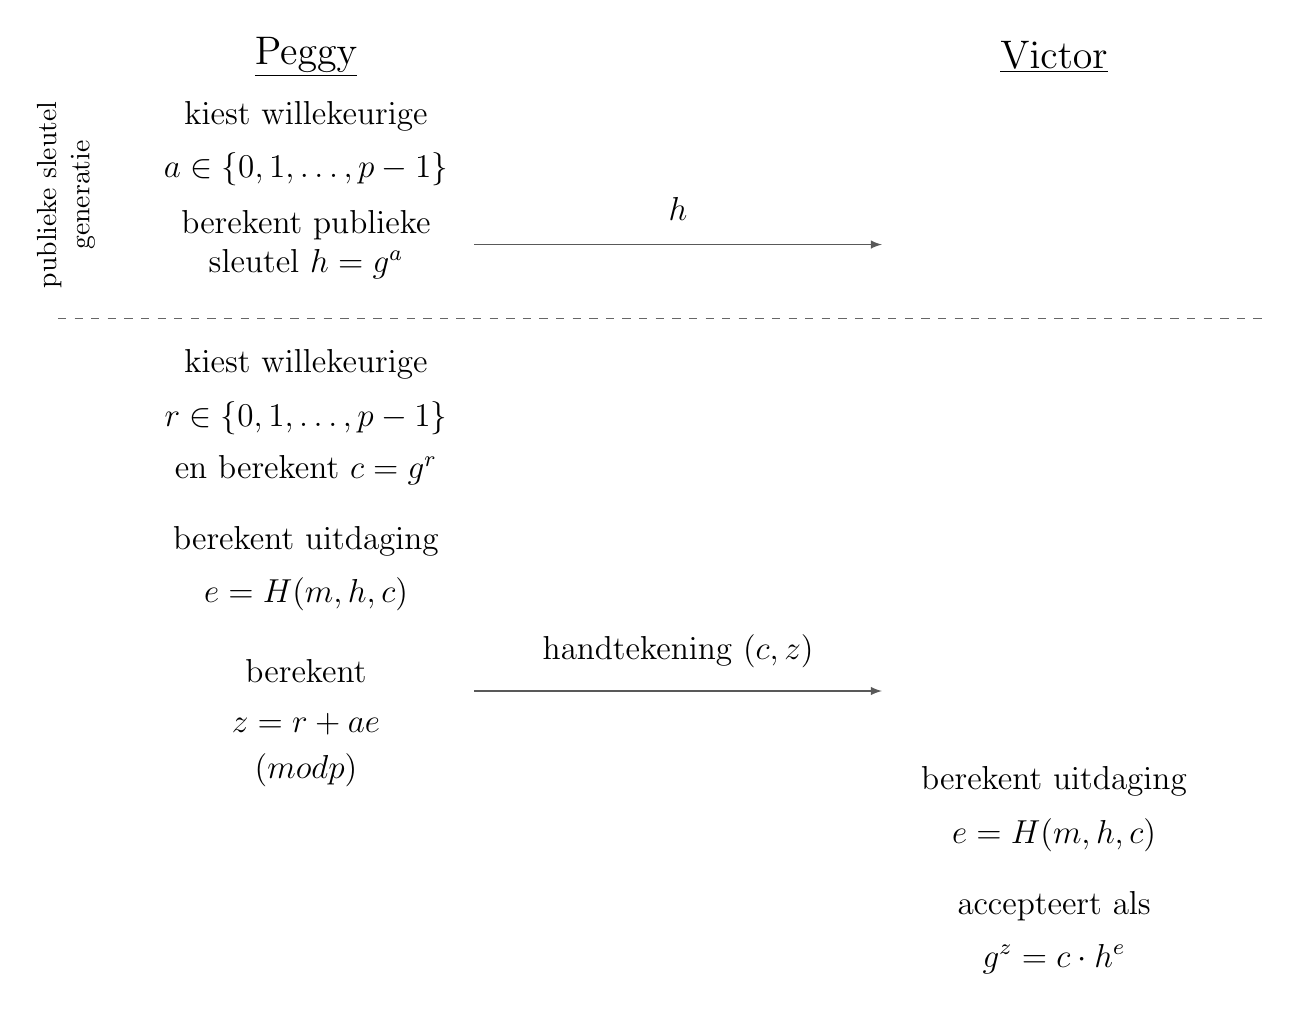
\begin{tikzpicture}[
    >=latex,
    participant/.style={
        font=\Large
    },
    textline/.style={
        font=\large,
        align=center
    },
    formula/.style={
        font=\large
    },
    message/.style={
        ->,
        thin,
        draw=black!65,
        shorten >=1pt,
        shorten <=1pt
    },
    separator/.style={
        dashed,
        thin,
        draw=black!60
    }
]

% Horizontale posities
\def\PeggyX{0}
\def\VictorX{9.5}

% ==================================================
% Deelnemers
% ==================================================

\node[participant] at (\PeggyX,6.1)
    {\underline{Peggy}};

\node[participant] at (\VictorX,6.1)
    {\underline{Victor}};

% ==================================================
% Publieke-sleutelgeneratie
% ==================================================

\node[
    rotate=90,
    font=\normalsize,
    align=center
] at (-3.05,4.35)
    {publieke sleutel\\generatie};

\node[textline] at (\PeggyX,5.35)
    {kiest willekeurige};

\node[formula] at (\PeggyX,4.68)
    {$a\in\{0,1,\ldots,p-1\}$};

\node[textline] at (\PeggyX,3.72)
    {berekent publieke\\sleutel $h=g^a$};

% Peggy stuurt de publieke sleutel naar Victor
\draw[message]
    (2.10,3.72)
    --
    node[above=5pt, formula] {$h$}
    (7.35,3.72);

% ==================================================
% Scheidingslijn
% ==================================================

\draw[separator]
    (-3.15,2.78) -- (12.15,2.78);

% ==================================================
% Commitment
% ==================================================

\node[textline] at (\PeggyX,2.20)
    {kiest willekeurige};

\node[formula] at (\PeggyX,1.52)
    {$r\in\{0,1,\ldots,p-1\}$};

\node[textline] at (\PeggyX,0.85)
    {en berekent $c=g^r$};

% ==================================================
% Uitdaging door Peggy
% ==================================================

\node[textline] at (\PeggyX,-0.05)
    {berekent uitdaging};

\node[formula] at (\PeggyX,-0.72)
    {$e=H(m,h,c)$};

% ==================================================
% Respons
% ==================================================

\node[textline] at (\PeggyX,-1.70)
    {berekent};

\node[formula] at (\PeggyX,-2.37)
    {$z=r+ae$};

\node[formula] at (\PeggyX,-2.95)
    {$(\operatorname{mod}p)$};

% Peggy stuurt de handtekening naar Victor
\draw[message]
    (2.10,-1.95)
    --
    node[above=5pt, formula]
    {handtekening $(c,z)$}
    (7.35,-1.95);

% ==================================================
% Verificatie door Victor
% ==================================================

\node[textline] at (\VictorX,-3.10)
    {berekent uitdaging};

\node[formula] at (\VictorX,-3.78)
    {$e=H(m,h,c)$};

\node[textline] at (\VictorX,-4.68)
    {accepteert als};

\node[formula] at (\VictorX,-5.35)
    {$g^z=c\cdot h^e$};

\end{tikzpicture}